\section{Nuclear Hamiltonians}\label{nuclear}
There are three additional contributions to the Hamiltonian to be considered which involve an interaction with the nucleus.

%
\subsection{\index{Zeeman!nuclear zeeman}{Nuclear Zeeman}}
Equivalent to electron Zeeman interaction but for the nuclear magnetic moment.\begin{equation}
	H_{\ce{Zeeman(n)}} = -g_n \mu_n \vec{B} \cdot \hat{\vec{I}}
	\label{eq:nuclear_zeeman_hamiltonian}
\end{equation}
 It is clear that this contribution is not spin-dependent, therefore it will manifest as a global energy shift and is not of interest for EPR. For this reason, the nuclear Zeeman interaction contribution will not be included for the remainder of this work. 

\subsection{\index{nuclear quadrupole}{Nuclear Quadrupole}}
Equivalent to the electron dipole-dipole but for nuclear magnetic moments.
\begin{equation}
	H_{\ce{Quadrupole}} = \hat{\vec{I}} \cdot Q \cdot \hat{\vec{I}}
	\label{eq:nuclear_quadrupole}
\end{equation}

 As for the nuclear Zeeman interaction, this contribution is not spin-dependent and the contribution will not be included for the remainder of this work. 

\subsection{\index{hyperfine interaction}{Hyperfine Interaction}}
% \begin{wrapfigure}{l}{0.4\textwidth}%
% 	\centering%
% 	% \begin{center}
% 	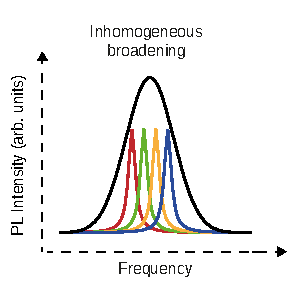
\includegraphics[width=0.38\textwidth]{figures/inhom-broadening.pdf}%
% 	% % MAGNETIC MOMENT ELECTRON + SPIN
\begin{tikzpicture}[thick, scale=1.5]
  \def\re{0.3}
  \def\ang{80}
  %\draw[dashed] (\ang-180:2.5*\re) -- (\ang:3.5*\re);
  \draw[mu vector] (0,0) -- (\ang+180:3*\re) node[right] {$\vb*{\mu}_\mathrm{B}$};
  \draw[spin] (0,0) -- (\ang:2.8*\re) node[right] {$\vb{S}$};
  \draw[charge-]
    (0,0) circle (\re) node[scale=1.4] {$-$}
    node[right=0.5] {$\mathrm{e}^-$};
  \draw[->,rotate=\ang-90]
    (0,-0.2*\re)++(-175:{1.6*\re} and {1.3*\re}) arc (-175:-35:{1.6*\re} and {1.3*\re})
    --++ (50:0.3*\re);
\end{tikzpicture}

% 	% \end{center}
% 	\caption{\cite{Rain2022}\td{write caption}}\label{fig:}
% \end{wrapfigure}
Equivalent to Fine Structure (ZFS) but between the nuclear and electron moment.
\begin{equation}
	H_{\ce{Hyperfine}} = \hat{\vec{S}} \cdot A \cdot \hat{\vec{I}}
	\label{eq:hyperfine_hamiltonian_dense}
\end{equation}
\begin{equation}
	H_{\ce{Hyperfine}} = A_\parallel \hat{S}_z\hat{I}_z + A_\perp(\hat{S}_y\hat{I}_y + \hat{S}_z\hat{I}_z)
	\label{eq:hyperfine_hamiltonian_componentwise}
\end{equation}
For the systems discussed in this work, hyperfine couplings are usually too small to detect,
thus manifest as inhomogeneous line broadening \cite{SpinStates}. We therefore do not include the hyperfine contribution
for the remainder of this work.
 \begin{figure}[H]
    \begin{center}
        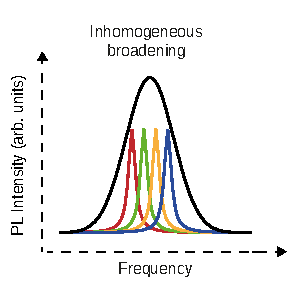
\includegraphics[width=0.5\textwidth]{figures/inhom-broadening.pdf}
        % \missingfigure{Figure showing line broadening due to hyperfine splitting}
	\caption{Illustration of the inhomogeneous line broadening caused by the hyperfine interactions. The individual resonances sum to a broader, brighter peak \cite{Rain2022}.}\label{fig:}
    \end{center}
\end{figure}



% \subsection{Nuclear Summary}
% We have chosen to include the nuclear Hamiltonians for completeness, but will now disregard them in the rest of this work since.
